\documentclass[parskip]{scrartcl}
\usepackage[margin=15mm]{geometry}
\usepackage{tikz}
\usetikzlibrary{snakes,decorations.pathreplacing}
\usetikzlibrary{patterns}

\newcommand{\flux}{yellow!75!gray}
\newcommand{\rightcoil}{green!85!gray}
\pgfmathsetmacro{\coilStart}{7}
\pgfmathsetmacro{\coilEnd}{8}

\begin{document}
%~~~~~~~~~~~~~~~~~~~~~~~~~~~~~~~~~~~~~~~~
% ELEC 467 Electric Machines and Transformers
% AC Electromagnetic Relay Diagram
% Written by Sze "Ron" Chau, October 2014
%
%~~~~~~~~~~ CHANGES FROM DC~~~~~~~~~~~~~~
% added grid line, comment out at completion
% use y=mx+b to establish the layout
% it's a mess, but to be fair I just got off
% from working a Code Blue all night. Yay hospital.
%~~~~~~~~~~~~~~~~~~~~~~~~~~~~~~~~~~~~~~~~
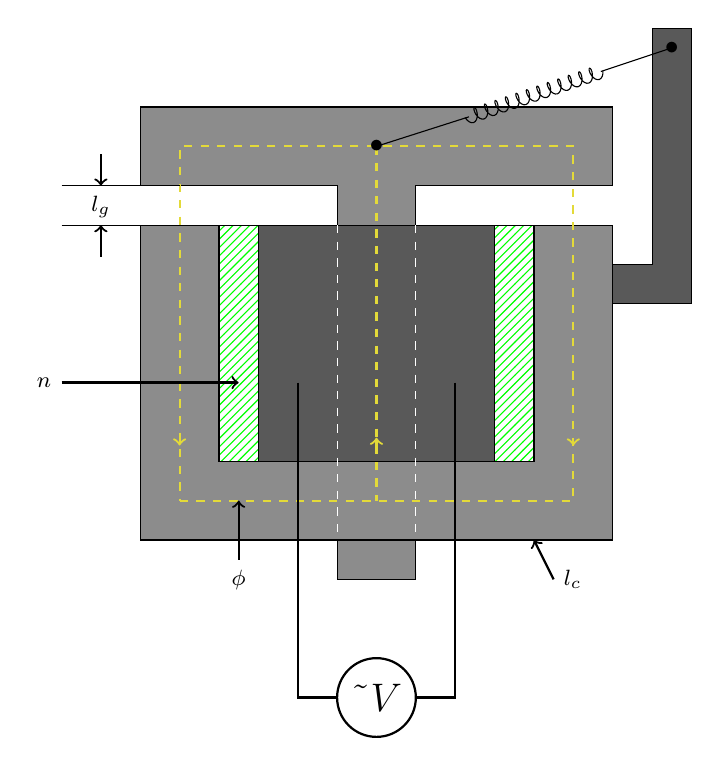
\begin{tikzpicture}

% GRID LINES - COMMENT OUT WHEN DONE
%\draw[step=1,gray,very thin] (-2,-2) grid (9,9);
%\foreach \x in {0,1,2,3,4}
%    \draw (\x cm,1pt) -- (\x cm,-1pt) node[anchor=north] {$\x$};
%\foreach \y in {0,1,2,3,4}
%    \draw (1pt,\y cm) -- (-1pt,\y cm) node[anchor=east] {$\y$};

% relay
\filldraw[fill=gray!90!white, draw=black](2,1) -- 
    (8,1) -- (8,5) -- (7,5) -- (7,2) -- (3,2) --
    (3,5) -- (2,5) -- cycle;
\filldraw[fill=gray!90!white, draw=black](2,5.5) --
    (4.5,5.5) -- (4.5,5) -- (5.5,5) -- (5.5,5.5) --
    (8,5.5) -- (8,6.5) -- (2,6.5) -- (2,6) -- cycle;
\filldraw[fill=gray!90!white, draw=black](4.5,1) --
    (4.5,0.5) -- (5.5,0.5) -- (5.5,1) -- cycle;

% center
\filldraw[fill=gray!70!black, draw=black] (3.5,5) --
    (3.5,2) -- (6.5,2) -- (6.5,5) -- cycle;
\draw[dashed,draw=white](4.5,5) -- (4.5,1);
\draw[dashed,draw=white](5.5,5) -- (5.5,1);

% plate
\filldraw[fill=gray!70!black, draw=black](8,4) -- (9,4) --
    (9,7.5) -- (8.5,7.5) -- (8.5,4.5) -- (8,4.5) -- cycle;

% flux lines
\draw[thick,dashed,draw=\flux]  (2.5,1.5) -- (7.5,1.5) --
    (7.5,6) -- (2.5,6) -- cycle;
\draw[thick,dashed,draw=\flux](5,6) -- (5,1.5);
\draw[thick,->,draw=\flux](5,2.15) -- (5,2.3);
\draw[thick,<-,draw=\flux](2.5,2.2) -- (2.5,2.3);
\draw[thick,<-,draw=\flux](7.5,2.2) -- (7.5,2.3);
\draw[thick,->](3.25,0.75)
    node[below]{\footnotesize$\phi$} -- (3.25,1.5);

% spring
\node(top) at (8.75,7.25){$\bullet$};
\node(bottom) at (5,6){$\bullet$};
\draw(8.75,7.25) -- (7.85,6.95);
\draw(5,6) -- (6.175,6.375);
\node(springTop)    at (8,7){};
\node(springBottom) at (6,6.315){};
\draw[snake=coil,segment length=4pt]
     (springTop) -- (springBottom);

% lengths of air gap and core
\draw(1,5) -- (2.5,5);
\draw(1,5.5) -- (2.5,5.5);
\draw[thick,->](1.5,5.9) -- (1.5,5.5) 
    node[below]{\footnotesize$l_{g}$};
\draw[thick,->](1.5,4.6) -- (1.5,5);
\draw[thick,->](7.25,0.5) 
    node[right]{\footnotesize$l_{c}$} -- (7,1);

% coils
\draw[pattern=north east lines,pattern color=green]
    (3,2) rectangle (3.5,5);
\draw[pattern=north east lines,pattern color=green]
    (6.5,2) rectangle (7,5);
\draw[thick,->](1,3) 
    node[left]{\footnotesize$n$} -- (3.25,3);

% power supply
\draw[thick](4,3) -- (4,-1) -- (4.5,-1);
\draw[thick](6,3) -- (6,-1) -- (5.5,-1);
\draw[thick](5,-1) circle (.5)
    node{\Large\textasciitilde $V$};

\end{tikzpicture}

\end{document}